\documentclass[10pt,a4paper]{article}
\usepackage[utf8]{inputenc}
\usepackage[czech]{babel}
\usepackage[T1]{fontenc}
\usepackage{amsmath}
\usepackage{amsfonts}
\usepackage{amssymb}
\usepackage{delarray}
\usepackage{float}

% exercises and solutions
\usepackage{mdframed}
\newmdenv[topline=false, bottomline=false, skipabove=\topsep, rightline=false,
  skipbelow=\topsep]{exercise}

% graphs
\usepackage{tikz}
%\usetikzlibrary[todraws]

\usepackage[left=2cm,right=2cm,top=2cm,bottom=2cm]{geometry}

\title{B4M36SAN - Statistická analýza, modely a jejich hodnocení. Redukce dimenze. Shlukování.}
\date{}
\begin{document}
\maketitle

\section{Redukce dimenze}

Při redukci dimenze chceme data dostat do nižší dimenze, např. kvůli vizualizaci nebo zmenšení při přenosu. Předpokladem je, že máme body $X = {x_i}$ z nějakého prostoru dimenze $D$. Předpokládáme, že $X$ leží aspoň přibližně na manifoldu dimenze $d < D$, kde $d$ je intrinsická dimenze.

Manifold je topologický prostor, na kterém můžeme měřit Euklidovské vzdálenosti s malou chybou. Manifoldem dimenze 1 je nějak zkroucená křivka v prostoru vyšší dimenze (ale ne osmička, protože uprostřed se kříží), manifoldem dimenze 2 je např. rovina zkroucená do rolády. Předpoklad toho, že data leží na manifoldu nižší intrinsické dimenze je důležitý proto, že kdyby na manifoldu neležela, pak nemá smysl redukovat dimenzi (protože se to nepovede).

Intrinsická dimenze popisuje, kolik proměnných je potřeba k popisu dat. Libovolný bod v $\mathbb{R}^3$ lze popsat třemi proměnnými, ale pokud víme, že leží na nějaké konkrétní přímce (nebo nějaké křivce), třeba na jedné z os, stačí nám proměnná jedna.

Výstupem Redukce dimenze je nový prostor nižší dimenze než $D$, a dvě mapovací funkce: z původního prostoru do toho redukovaného, a z redukovaného prostoru do toho původního.

\subsection{PCA - Principal Component Analysis}

PCA najde největší varianci a transformuje data tak, aby byla ve směru osy. Toho dosáhne tak, že diagonalizuje kovariační matici. Data nejprve \textit{posuneme do počátku}.

\begin{equation}
X = 
\left( \begin{array}{ccc}
1 & 1 & 1\\
1 & 2 & 1\\
1 & 3 & 2\\
1 & 4 & 3 \end{array} \right)
%
\sim
%
\left( \begin{array}{ccc}
0 & -1.5 & -0.75\\
0 & -0.5 & -0.75\\
0 & 0.5 & 0.25\\
0 & 1.5 & 1.25 \end{array} \right)
\end{equation}
Kovariační matici spočítáme tak, že na každou dvojici příznaků použijeme vzorec pro $\text{cov}(X, Y)$, a tím nám vznikne symetrická matice. Protože $E(X)$ všech příznaků je 0, tak se to dá zjednodušit na $C_X = \frac{1}{m}X^TX$.

\begin{equation}
\text{cov}(X,Y) = \frac{1}{n} \sum_{i=1}^n (x_i-E(X))(y_i-E(Y))
\end{equation}

Protože je kovariační matice symetrická, můžeme ji rozložit jako $C_X = P\Lambda P^{-1}$, kde $P$ má ve sloupcích vlastní vektory $C_X$ a $\Lambda$ je matice vlastních čísel. Protože $P$ je ortogonální, pak $P^{-1}=P^T$, a $P$ je zároveň transformační maticí, kterou hledáme.

\subsection{Kernel PCA}

PCA funguje dobře pro lineární data. Pokud máme data např. na kružnici, tak je PCA k ničemu. Chceme najít funkci $\Phi$, která data nejprve nějak upraví, aby šla lépe zpracovat (třeba $\mu_1 = x_1^2, \mu_2 = x_2^2$ pro kružnici, protože předpis kružnice je $x^2+y^2=1$).

Využijeme toho, že v PCA jsme pracovali s daty $X$ jen jako se skalárním součinem $X^TX$. Zvolíme kernel funkci $K$. Pokud chceme běžné PCA, pak bude rovna skalárnímu součinu: $K(x_i, x_j) = \langle x_i, x_j\rangle$. Můžeme ale zvolit jiné funkce (které musí splňovat nějaké vlastnosti) a pak můžeme postupovat stejně jako u PCA, jen počítáme $C_X = \frac{1}{m}K$.

Vhodnou kernel funkcí je např. RBF (radial basis function). KPCA funguje dobře i na nelineární manifoldy, a jeho složitost neroste s dimenzí dat (protože redukce dimenze se děje už v $K$). Nevýhodou je, že je těžké až nemožné získat funkci pro zpětnou transformaci dat.

\subsection{MDS - MultiDimensional Scaling}

Hlavní myšlenkou MDS je, že body, které jsou blízko sebe, mají zůstat blízko, a vzdálené body mají zůstat daleko od sebe. Řešíme úlohu, kde minimalizujeme stresovou funkci:

\begin{equation}
\text{stress}(T, f)=\sqrt{\frac{\sum_{i,j=1}^m(f(\delta_{ij})-d_{ij})^2}{\sum_{i,j=1}^m d_{ij}^2}}
\end{equation}

\noindent kde $T$ jsou data, $f$ je transformační funkce, a $d_{ij}$ a $\delta_{ij}$ jsou vzdálenosti v původním a novém prostoru.

Pro vhodný výpočet vzdálenosti na manifoldu můžeme použít funkci \textbf{Isomap}. V ní se sestaví graf (síť) nejbližších bodů, např. zohledněním okolí nebo nalezení $k$ nejbližších sousedů. Pak se spočítají euklidovské vzdálenosti mezi přímými sousedy, a vzdálenosti dalších bodů se získají jako délka nejkratší cesty grafem (součet euklidovských vzdáleností). 


\subsection{LLE - Locally Linear Embedding}

Každý bod vyjádříme jako lineární kombinaci sousedů, s nějakými váhami. Chceme, aby po transformaci zůstaly tyto váhy zachovány. Řešíme pak úlohu lineárního programování.

Výhodou LLE je, že jediným parametrem je počet sousedů, a je efektivní i pro velké datové sady. Nevýhodou je, že metoda není stabilní v řídkých oblastech, a pokud se do dat přidá nový bod, je potřeba vše spočítat znovu.

\subsection{t-SNE - t-Distributed Stochastic Neighbor Embedding}

Klade důraz na to, že malé vzdálenosti zůstanou podobné, u velkých povoluje větší změny. Vzdálenosti převedu na pravděpodobnosti (je pravdděpodobnější, že vytáhneme dva body, které jsou blízko sebe). Vzdálenost bodů $i$ a $j$ v původním prostoru bude nepřímo úměrná pravděpodobnosti $p_{ij}$, a v novém prostoru bude vzdálenost nepřímo úměrná pravděpodobnosti $q_{ij}$. Pak minimalizujeme Kullback-Leiblerovu divergenci:

\begin{equation}
S=KL(P||Q)=\sum_i\sum_{j\neq i} p_{ij}\text{log}\frac{p_{ij}}{q_ij}
\end{equation}

Ve slidech jsou obrázky, kde je vidět, že to dobře funguje na clusterování - třeba charakteristiky rukou psaných číslic tam jdou hezky rozdělit do skupin, protože důraz byl na to, aby podobné číslice zůstaly u sebe, a oddělení jednotlivých skupin nevadí.

\subsection{SOM - Self Organizing Map}
V sešitě o tom nic nemám a ze slidů to moc nechápu. Podle jednoho YT videa to vypadá, že se udělá síť s několika \textit{neurony} (zvolíme tolik neuronů, kolik očekáváme clusterů), a tu síť se snažíme napasovat na data:

\begin{enumerate}
\item Vybereme nějaký bod v datech
\item Najdeme nejbližší neuron, to je \textit{winner}, a síť posuneme/natáhneme tak, aby byl \textit{winner} blíž k vyubranému bodu
\item Jdeme na krok 1 a vybereme nový bod
\end{enumerate}

\noindent Na konci máme síť, kde každý neuron by měl být u jednoho clusteru dat. Je to dost podobné jako $k$-means.







\section{Shlukování}

Shlukování je zpracování dat, kdy se snažíme body rozdělit do $k>1$ tříd. Výsledkem je množina $\Omega = \{C_1, C_2, \dots, C_k\}$, kde $C_i$ jsou výsledné disjunktní shluky (množiny bodů). Vhodnou metodu budeme vybírat podle toho, jaká máme data: víme, kolik je shluků? Jak jsou shluky husté? Jaký mají shluky tvar?

\subsection{K-means}

\begin{enumerate}
\item Vyberu $k$ bodů z dat, klidně náhodně. Do nich umístím středy shluků.
\item U každého bodu v datech najdu, do kterého shluku patří (najdu nejbližší střed).
\item Každý střed posunu tak, aby ležel uprostřed svého shluku (tj najdu medián všech bodů, které přísluší k danému středu).
\item Opakuju body 2 a 3, dokud se středy mění.
\end{enumerate}

K-means vždycky skončí, protože součet vzdáleností bodů od středů se v kroku dva zmenší, a v kroku 3 zůstává stejný, a nemůžeme zmenšovat do nekonečna. Algoritmus může ale uváznout v lokálním minimu - to se obvykle řeší tak, že vybereme nejlepší výsledek z několika náhodně inicializovaných běhů.

Můžeme použít různé vzdálenostní funkce a bude to fungovat taky. Důležité je vybrat správné $k$. To se dá dělat tak, že spustím algoritmus pro různá $k$, a počítám nehomogenitu $W(k)$ (součet vzdáleností bodů od středů). Všechna $W(k)$ zakreslím do grafu a zvolím takové $k$, na kterém nehomogenita náhle klesla a dál už neklesá - graf tam vypadá jako pata. Další možností je $W(k)$ dále zpracovat a spočítat z něj Hartiganovo kritérium.

Variantou k-means je kernel k-means, kde nejprve body převedeme kernel funkcí a jejich vzdálenosti počítáme v jiném prostoru. Tím pak jdou shlukovat i data, která nejsou lineárně separovatelná.

\subsection{EM - Expectation Maximization}

Je složitý, vzorce nechápu, a proto sem dávám jen intuitivní popis. EM je hodně podobný algoritmu k-means co se týče postupu a kroků, ale liší se v tom, jak se body přiřazují do shluků. V k-means bylo přiřazení ostré: každý bod patří přesně do jednoho shluku, a shluk je definovaný svým středovým bodem. V EM jsou \textit{středy shluků} pravděpodobnostní rozdělení, která mají $\mu$ a rozptyly (v případě Gaussů). Pak nezjišťujeme, do kterého shluku bod patří, ale s jakou pravděpodobností patří do každého shluku (Expectation). V druhé fázi (Maximization) pak hledáme nové a lepší parametry shluků metodou MLE (Maximal Likelihood Estimation).

Výhodou EM oproti k-means je to, že na konci máme rozdělení, a můžeme generovat nové vzorky dat. Shluky taky můžou mít různé tvary.


\subsection{Hierarchické shlukování}

Data shlukujeme na základě podobnosti, nemusíme předem znát počet shluků. První možnost je začít s jedním shlukem a ten dělit na menší (to je sice efektivní, ale složité, a dál se tím nebudeme zabývat). Druhá možnost je umístit každý bod do vlastního shluku, postupně spojovat podobné shluky. Vzniká přitom strom - dendrogram, kde je vidět, jak se postupně shluky spojují, dokud nemáme jeden velký shluk.

\begin{figure}[ht!]
\centering
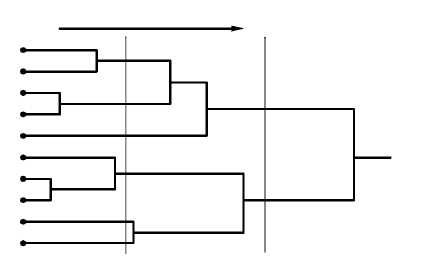
\includegraphics{img/dendrogram.png}
\end{figure}

Na základě dendrogramu se můžeme rozhodnout, kde shlukování zastavíme, udělat tam svislou čáru a tím určit počet shluků. Na obrázku máme svislé čáry dvě, jednou vznikne 6 shluků, druhou pouze dva shluky. \textit{Výška} v dendrogramu znázorňuje vzdálenost shluků

Pro tento typ shlukování je zásadní, jak počítáme vzdálenost shluků:
\begin{itemize}
\item \textbf{Single linkage} Vzdálenost shluků je rovna vzdálenosti dvou nejbližších bodů ve shlucích
\item \textbf{Complete linkage} Vzdálenost shluků je rovna vzdálenosti dvou nejvzdálenějších bodů ve shlucích
\item \textbf{Average linkage} Vzdálenost shluků získáme jako průměr vzdáleností všech dvojic bodů
\item \textbf{Centroid} Vzdálenost shluků získáme jako vzdálenost jejich středů
\end{itemize}

Vliv výpočtu vzdáleností shluků je patrný na obrázku níže, kde pracujeme s jednodimenzionálními daty: 2, 12, 16, 25, 29, 45.

\begin{figure}[ht!]
\centering
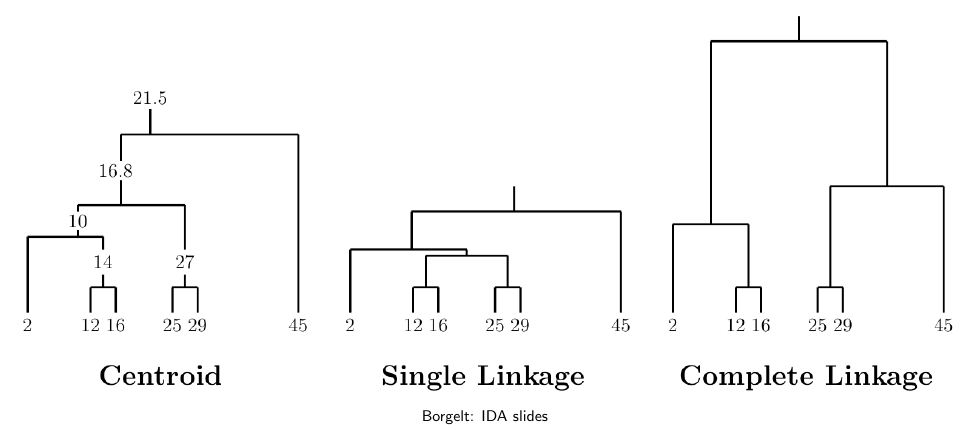
\includegraphics[width=\textwidth]{img/dendrogram-example.png}
\end{figure}

\subsection{Shlukování podle hustoty}

Předpokládáme, že shluky budou mít vyšší hustotu a budou odděleny místy, kde je hustota nižší. Výhodou takového algoritmu je, že nepotřebuje $k$ a umí najít i shluky, které jsou do sebe zamotané, třeba dvě spirály. Naopak problém je, pokud mají shluky různou hustotu.

Shlukování podle hustoty dělá algoritmus DBSCAN. Ten potřebuje dva parametry: velikost okolí a počet sousedů v husté oblasti. Body pak dělí do tří skupin: bod uvnitř shluku (má dost sousedů), hraniční bod (nemá dost sousedů, ale jeho přímí sousedi jsou uvnitř shluku) a bod mimo shluk (nemá dost sousedů, a nesousední s body uvnitř shluku). Výstupem jsou shluky a pak seznam bodů mimo ně.

\subsection{Spektrální shlukování}

Z dat vytvořím síť (graf) a postupně odebírám ty nejdelší hrany. Výsledkem je několik oddělených komponent (shluků). Pro jednoduchost budu pracovat s grafem, ve kterém jsou patrné dvě komponenty (jak se pracuje s body a ne z grafem je popsané níže).

\begin{figure}[ht!]
\centering
\begin{tikzpicture}
    \node[shape=circle,draw=black] (A) at (0,1) {A};
    \node[shape=circle,draw=black] (B) at (0,0) {B};
    \node[shape=circle,draw=black] (C) at (1, 0.5) {C};
    \node[shape=circle,draw=black] (D) at (2.5, 0.5) {D};
    \node[shape=circle,draw=black] (E) at (3.5, 1) {E};
    \node[shape=circle,draw=black] (F) at (3.5, 0) {F} ;

    \draw(A) to (B);
    \draw(B) to (C);
    \draw(A) to (C);
    \draw(D) to (C);
    \draw(D) to (E);
    \draw(D) to (F);
    \draw(E) to (F);   
\end{tikzpicture}
\end{figure}

Nejprve určím matici $S$, kde je jednička, pokud z vrcholu $i$ do vrcholu $j$ vede hrana. Protože je graf neorientovaný, bude matice symetrická. Pokud bychom nepracovali s grafem ale s body, tak matice $S$ bude \textit{similiarity}-matrix, kde počítáme blízkost bodů Gaussovým kernelem (čím bližší body, tím vyšší hodnota) a pak prahujeme podle nějaké konstanty. Tak jako tak vznikne symetrická matice.

Kromě matice $S$ sestavíme taky matici $D$, která bude mít na diagonále stupně vrcholů a jinak bude nulová (tedy je taky diagonální). Z nich spočítáme Laplacián grafu, $L = D - S$.

\begin{equation}
S = 
\left( \begin{array}{cccccc}
0 & 1 & 1 & 0 & 0 & 0\\
1 & 0 & 1 & 0 & 0 & 0\\
1 & 1 & 0 & 1 & 0 & 0\\
0 & 0 & 1 & 0 & 1 & 1\\
0 & 0 & 0 & 1 & 0 & 1\\
0 & 0 & 0 & 1 & 1 & 0\end{array} \right)
%
,
%
D = 
\left( \begin{array}{cccccc}
2 & 0 & 0 & 0 & 0 & 0\\
0 & 2 & 0 & 0 & 0 & 0\\
0 & 0 & 3 & 0 & 0 & 0\\
0 & 0 & 0 & 3 & 0 & 0\\
0 & 0 & 0 & 0 & 2 & 0\\
0 & 0 & 0 & 0 & 0 & 2\end{array} \right)
%
,
%
L = 
\left( \begin{array}{cccccc}
2 & -1 & -1 & 0 & 0 & 0\\
-1 & 2 & -1 & 0 & 0 & 0\\
-1 & -1 & 3 & -1 & 0 & 0\\
0 & 0 & -1 & 3 & -1 & -1\\
0 & 0 & 0 & -1 & 2 & -1\\
0 & 0 & 0 & -1 & -1 & 2\end{array} \right)
\end{equation}

K matici $L$ spočítáme vlastní čísla a vlastní vektory (postup je rozepsaný na webu v QR kódu), a vyjdou čtyři vlastní čísla a vektory:


\begin{figure}[H]
\centering
\begin{minipage}{0.15\textwidth}
\centering

\includegraphics[width=\textwidth]{img/spectral-clustering-qr}
\end{minipage} \hfill
\begin{minipage}{0.84\textwidth}

$\lambda_1 = 0, v_1 = (1, 1, 1, 1, 1, 1)$\\
$\lambda_2 \doteq 0.44, v_2 = (-1, -1, -0.56, 0.56, 1, 1)$\\
$\lambda_3 = 3, v_3 = (-1, 1, 0, 0, 0, 0)$\\
$\lambda_4 \doteq 4.56, v_4 = (-1, -1, 3.56, -3.56, 1, 1)$\\


\end{minipage}
\end{figure}

Teď jsou dva způsoby, jak z toho dostat shluky. Na přednášce jsme si říkali, že vektory dáme jako sloupce do matice $V$, a pak v řádcích té matice máme body. Na ně spustíme nějaké rychlé shlukování, třeba k-means. V přednáškách ze Stanfordu na to jdou ještě lépe, vezmou vektor odpovídající druhému nejmenšímu vlastnímu číslu (to nejmenší je nula a to je nuda), tedy v našem případě $v_2 = (-1, -1, -0.56, 0.56, 1, 1)$. Pak řeknou, že body, kterým přísluší záporné hodnoty (A, B, C) jsou jeden shluk a zbylé body jsou druhý shluk (D, E, F). Pokud chtějí víc clusterů, tak zpracovávají vektor $v_2$, někdy tam je těch úrovní zřetelných víc.


\section{Multivariátní analýza}

\subsection{ANOVA - Analýza rozptylu}

Zjišťujeme, jestli můžeme zamítnout hypotézu $H_0$: průměry ve všech skupinách dat jsou stejné (např. ženy, muži i děti mají stejnou výšku v cm). Mohli bychom to dělat třeba nepárovým t-testem na dvojici vzorků (párový t-test porovnává stejná data před a po, např. náladu lidí před vypitím kafe a po něm). Problém je, že pokud budeme dělat t-test pro každou dvojici skupin, tak to bude časově náročné pro hodně skupin, a taky tam bude víc chyb.

ANOVA předpokládá, že v každé skupině mají data normální rozdělení, že jsou nezávislá, a všechny skupiny mají stejný rozptyl. Zkoumáme vždy právě jednu proměnnou.

Zkusím to na třech třídách dat, $A = \{1, 2, 5\}, B = \{2, 4, 2\}, C = \{2, 3, 4\}$. Nulová hypotéza je, že všechny skupiny mají stejnou střední hodnotu. Všechno v postupu počítáme dvakrát, jednou mezi třídami (between) a pak uvnitř tříd (within). Názvy Ve slidech se to značí treat a error, což mě mátlo, a tak to sem psát nebudu.

Stupně volnosti jsou: $DF_{\text{between}} = k - 1 = 3-1 = 2, DF_{\text{within}} = N - k = 9 - 3 = 6$, kde $N$ je počet datových bodů, a $k$ je počet tříd. Pomocí stupňů volnosti najdeme tabulkovou $F$ hodnotu, $F_{\text{crit}} = 5.14$.

Spočítáme střední hodnota pro skupiny: $\mu_A=2.67,\mu_B=2.67,\mu_C=3$ a celkový průměr $\mu=2.78$. Počítáme \textit{Sum of Squares} ($SS$). Celkový $SS$ je součet vzdáleností všech bodů od střední hodnoty, a má dvě součásti: uvnitř skupiny a mezi skupinami. Sumy nejsou korektně značené, total se počítá pro všechna data, a within pro všechna data, ale odděleně po třídách.

\noindent $SS_\text{total} = \sum (x - \mu)^2 = (1-2.78)^2 + (2-2.78)^2 + (5-2.78)^2 + (2-2.78)^2 + (4-2.78)^2 + (2-2.78)^2 + (2-2.78)^2 + (3-2.78)^2 + (4-2.78)^2  = 13.6$

\noindent $SS_\text{within} = \sum (x - \mu_X) = (1-2.67)^2 + (2-2.67)^2 + (5-2.67)^2 + (2-2.67)^2 + (4-2.67)^2 + (2-2.67)^2 + (2-3)^2 + (3-3)^2 + (3-4)^2 = 13.34$

\noindent $SS_\text{between} = SS_\text{total} - SS_\text{within} = 13.6 - 13.34 = 0.23$

Dál počítáme \textit{rozptyly}:

\noindent $MS_\text{between} = \frac{SS_\text{between}}{DF_text{between}} = \frac{0.23}{2} = 0.12$

\noindent $MS_\text{within} = \frac{SS_\text{within}}{DF_text{within}} = \frac{13.34}{6} = 2.22$

Spočítáme $F$ hodnotu, $F=\frac{MS_\text{between}}{MS_\text{within}} = \frac{0.12}{2.22} = 0.05$

Protože $F<F_\text{crit}$, tedy $0.05 < 5.14$, tak nemůžeme nulovou hypotézu zamítnout, tedy je možné, že všechny skupiny mají stejnou střední hodnotu. F rozdělení je podíl dvou $\chi^2$ rozdělení.

Pokud by ANOVA nulovou hypotézu zamítla, tak pak by se třeba hodilo vědět, která ze skupin má odlišnou střední hodnotu. To nám ale ANOVA říct neumí, a musíme to zjistit jinak, třeba Tukeyho HSD testem. ANOVA umí pracovat pouze s jednou proměnnou, a pracuje s nezávislými měřeními.

\subsection{MANOVA}

Funguje podobně jako ANOVA, ale umožňuje víc náhodných veličin. Předpokladem je, že rozdělení jsou normální a mají napříč třídami stejné kovariační matice, jsou náhodně vzorkované atd, jako u ANOVy. Pro $p$ náhodných veličin vzniknou místo dvou hodnot $SS$ z ANOVy dvě matice $E$ a $H$ z $\mathbb{R}^p$. Pak ve vzorci není $(x - \mu)^2$, ale $(x_i - \mu_i)(x_j - \mu_j)$. Výsledek MANOVY se zpracuje Wilkovým lambda testem (nebo něčím jiným).







\section{Regrese}

\subsection{Lineární regrese}

Chceme data proložit přímkou (nebo rovinou). Předpokládáme, že data jsou lineární a že chyba od dat má normální rozdělení. I přes to, že jsou předpoklady nereálné, to dobře funguje. Pracujeme s modelem $Y = \beta_0 + \beta_1 X + \varepsilon$, kde $\beta$ jsou parametry, které hledáme, a $\varepsilon$ je chyba nebo šum.

Spočítáme RSS (Residual sum of squares) jako součet všech chyb: $RSS = \sum (y_i - \beta_0 - \beta_1x_1)^2$. RSS pak minimalizujeme, abychom dostali optimální parametry $\beta$.

Např. chceme proložit body: $[1, 3], [2,4], [3,5], [4, 4], [5,4], [6,5], [7,6], [8,7]$. Pro jednoduchost přejmenujeme parametry $\beta$, takže pracujeme se vztahem $y = a + bx + \varepsilon$. Vypočítáme $RSS = \sum (y_i - a - bx_i)^2 = (3-a-b)^2 + (4-a-2b)^2 + (5-a-3b)^2 + (4-a-4b)^2 + (4-a-5b)^2 + (5-a-6b)^2 + (6-a-7b)^2 + (7-a-8b)^2 = \cdots = 192 - 76a -370b + 8a^2  + 72ab + 204b^2$.

Tím máme RSS, a to chceme minimalizovat. Nejmenší hodnota bude tam, kde je nulová derivace (tam se křivka zvedá zase zpět nahoru).


\begin{minipage}{0.45\textwidth}
\begin{equation}
\begin{split}
\frac{\partial{RSS}}{\partial{a}} = 0 \\
-76 +16a +72b = 0 \\
16a + 72b = 76 \\
4a + 18b = 19 \\
a = \frac{19 - 18b}{4}
\end{split}
\end{equation}
\end{minipage} \hfill
\begin{minipage}{0.45\textwidth}
\begin{equation}
\begin{split}
\frac{\partial{RSS}}{\partial{b}} = 0 \\
-185+36a+204b=0 \\
36a+204b=185 \\
36\frac{19-18b}{4} + 204b = 185 \\
171 -162b+204b = 185 \\
42b = 14\\
b = \frac{1}{3}\\
a = \frac{19-\frac{18}{3}}{4} = \frac{13}{4}
\end{split}
\end{equation}
\end{minipage}

Dostali jsme parametry přímky: $y = \frac{x}{3} + \frac{13}{4}$. Vyznačené svislé čáry směrem k přímce jsou chyby $\varepsilon$, které jsme minimalizovali.

\begin{figure}[ht!]
\centering
\begin{tikzpicture}
\draw[help lines, color=gray!30, dashed] (0, 0) grid (8.9,8.9);
\draw[->,ultra thick] (-0.2, 0)--(9,0) node[right]{$x$};
\draw[->,ultra thick] (0,-0.2)--(0,9) node[above]{$y$};

\foreach \x/\y in {1/3,2/4,3/5,4/4,5/4,6/5,7/6,8/7}{
	\draw[color=gray!60] (\x,\y)--(\x, 13/4+\x/3);
	\node at (\x,\y) {\textbullet};
}

% \foreach \Point in {(1, 3), (2,4), (3,5), (4, 4), (5,4), (6,5), (7,6), (8,7)}{
%     \node at \Point {\textbullet};
% }

\draw (-0.2, 3.183)--(8.9, 6.2167);

\end{tikzpicture}
\end{figure}

Jakmile máme parametry, tak můžeme měřit jejich chybu $SE$ pro každý z parametrů zvlášť, nebo RSE (residual standard error), což je odhad $\sigma$. Z hodnot $SE$ můžeme získat \textit{confidence intervaly}, které nám říkají, že s pravděpodobností $1-\alpha$ bude hodnota parametru ležet uvnitř toho intervalu. $SE(\beta_1)^2 = \frac{\sigma^2}{\sum_{i=1}^m(x_i-\bar{x})^2}$, kde jako $\sigma^2$ můžeme použít odhad $\sigma^2 = \frac{RSS}{m-2}$.

Testování hypotéz: Testujeme $H_0$, že není vztah mezi $X$ a $Y$, tedy $H_0: \beta_1 = 0$. Použijeme t-statistiku: $t = \frac{\beta_1 - 0}{SE(\beta_1)}$, kde za $\beta_1$ dosadíme parametr odhadnutý lineární regresí (a mně se nad něj nechce psát pořád stříšku). Má to $m-2$ stupně volnosti.

K hodnocení přesnosti modelu můžeme použít $R^2$, které nám říká, jaká část rozptylu v datech je vysvětlená modelem. $TSS = \sum_{i=1}^m(y_i - \bar{y})^2$ je celkový součet čtverců (vzdálenost od střední hodnoty), $RSS = \sum_{i=1}^m(y_i - \hat{y}_i)^2$ je vzdálenost bodů od odhadů. Pak $R^2 = \frac{TSS - RSS}{TSS}$.

Pokud chceme pracovat s vícedimenzionálním vstupem, přidáme další parametr beta:  $Y = \beta_0 + \beta_1 X_1 + \beta_2 X_2 + \varepsilon$. Pokud máme pocit, že se různé vstupy ovlivňují, např. zisk v závislosti na reklamu v televizi a reklamu v rozhlase, tak můžeme přidat ještě jeden parametr: $Y = \beta_0 + \beta_1 X_1 + \beta_2 X_2 + \beta_3 (X_1 X_2) + \varepsilon$ a pak zjišťujeme, které $\beta$ je nejvýznamnější.

\paragraph{Ridge regression}
Neminimalizujeme jen $RSS$, ale $RSS + \lambda\sum\beta_i^2$, tedy penalizujeme velká $\beta$, a parametr $\lambda$ určuje, jak přísně. To vede k tomu, že parametry $\beta$ budou co nejnižší, a tedy neužitečné proměnné se skoro nepoužijí ($\beta$ bude nula). Než se na datech spustí ridge regression, je vhodné data standardizovat (ve slidech je na to složitý vzorec, ale předpokládám, že to prostě od dat odečte střední hodnotu, aby byly v průměru na nule). Vhodný parametr $\lambda$ najdeme třeba cross-validací.

\paragraph{Lasso regression} Funguje stejně jako ridge regression, ale minimalizuje $RSS + \lambda\sum|\beta_i|$, tedy ne druhé odmocniny. Tím budou koeficienty u neužitečných prediktorů nejen malé, ale dokonce nulové, a budeme je moct úplně zahodit.

\subsection{Nelineární regrese}

















\end{document}
